\chapitre{Un sous-sol à Nazareth, le lundi 18 juillet 2033} {D'aucuns diraient}{ qu’il fait chaud pour mourir, que c’est sale partout, que ça sent le vieux, que la bonne femme est due pour un bain et le bonhomme, pour un récurage à la brosse. Mais à quoi cela servirait-il de le penser. «D’aucuns» n’existent pas, personne, sauf le fils, ne vient ici. Personne ! Jamais ! Et il ne peut en être autrement; c’est la nature même du châtiment. Personne ne peut imaginer venir ici parce que personne ne peut imaginer qu’il y habite des gens, enfin des vieux qui ne sourient jamais et qui se parlent que très rarement.}

À 82 ans, Marie Rioux est devenue «sec comme un balai» ; pas une once de graisse ne l’enrobe et son dos n’a pas encore commencé à voûter. «Rien à gruger su’ l’os», aurait dit son oncle Robert, autrefois plombier à Québec. Vêtue d’un vieux Levys foncé, ceux qu’elle préférait, et d’un antique coton ouaté commémorant la victoire de Barack Obama aux présidentielles américaines de 2008, elle s’occupe à faire luire le bois de son violoncelle. Autant le jeans que le chandail sont délavés, tout comme ses cheveux remontés en toque qui sont devenus blanc jaune. Ses pieds sont chaussés de bas de laine troués achetés, naguère, dans un surplus de l’armée. Ses mains sont longues, criblées de taches, bosselées par l’arthrite et ses ongles ne sont presque plus entretenus. D’ailleurs, pourquoi le ferait-elle? Pour qui ?

Son compagnon, cet être édenté, mal rasé, calé dans son lazy boy, les lèvres et la langue faisant «bleblebleblebleblebleble» à chaque respiration, se nomme Romain Tardif dit «le gelé». Il échappe la télécommande qui, sans bruit, choit sur le tapis moucheté de gris et de beige, un tissu fatigué dont la vocation est d’absorber poussières et petits détritus sur tous les planchers du sous-sol. L’homme se réveille en sursaut, convaincu d’avoir commis un impair majeur.

Assise juste à côté dans l’autre misérable fauteuil, la vieillarde le fixe de ses yeux superbes, des charbons qui n’ont pas vieilli, mais dont le potentiel de causticité, d’implacabilité et même de venimosité est demeuré aussi redoutable qu’il y a 53 ans. À ses pieds, la tête sur ses courtes pattes crochues, Gazou, un animal hargneux, mi-rat, mi-loulou obèse - ceux qui font “tic-tic-tic-tic” en marchant sur le prélart - une sale bête de chien jaune à poil ras et au nez brun avec, en tout temps, un croc saillant sur le museau, regarde avec haine la télécommande qui vient de le tirer de son sommeil. Sans rien dire, Marie reprend sa méticuleuse opération.

«Qu’elle était belle et séduisante», se remémore l’homme en s’étirant légèrement la jambe gauche, celle de son nerf sciatique. Puis, comme s’il eut voulu exaspérer davantage Marie et sa bête, il baille à s’arracher le maxillaire tout en son et lumière.

Étrangement, il a été épargné par la calvitie et sa tignasse blanche tout ébouriffée se termine en queue de cheval, laquelle date, selon toute apparence, du temps de sa moustache à la Frank Zappa, Sonny Bono ou Hulk Hogan. Le bonhomme est habillé d’un improbable short Nike, le modèle rouge à bandes noires sur les hanches, un short suspect taché d’on ne sait trop quoi, d’une camisole devenue jaune qui cache à peine ses chairs amollies, d’une paire de chaussettes bien étirées vers les mollets, des chaussettes ahurissantes à motifs de Schtroumpf, et de sandales avec semelles en retaille de pneu.

\begin{floatingfigure}[l]{40mm}
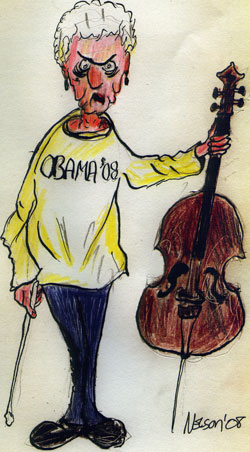
\includegraphics[height=60mm]{corps/chapitre1/img/maririou062.jpg}
\end{floatingfigure}

- Gajoo, rechte à côté de Maman, chinon, tu vas payer pour. Ta-tchu compris ?

Le chien jaune se replonge le mufle dans les pattes. De son œil hypocrite, il a vu que «Maman» ne blaguait pas et il se méfie de son archet.

Dans ce modeste logement de Nazareth, quartier s’étirant de Sacré-Cœur à la rivière Rimouski, on ne retrouve aucune photo sur les rares espaces que le rayonnage irrégulier de livres n’a pas volé aux murs. Ni de ces deux vieux assis la mâchoire pendante devant la télé, une antique HD aux couleurs déphasées, ni d’enfants potelés laissant paraître une dent au travers de leur sourire habituellement qualifié d’angélique, ni de scènes du «bon vieux temps d’avant le sida» alors que tout était si «désormais» facile, si «définitivement» cool, ni de fumeurs de cigarettes, oncles ou cousines depuis longtemps disparus, croqués en noir et blanc dans leurs vies de misère à la merci de la damnation éternelle, ni de guitaristes rock drapés dans le très pop Star-Spangled Banner. On ne retrouve aucune photo, pas plus qu’on ne remarque de reproductions de Toulouse-Lautrec, de nature morte peinte par la tante Hermance, cette vieille chipie de chez les Tardif, d’horloge Molson Export volée dans un hôtel de saint en arrière, d’écran plasma sans fil au récepteur défectueux, de feuilles de «pot» séchées et vernies, de poster du Che, de Dalida ou de Bob Dylan.

Plutôt, ici et là, une partition musicale imprimée sur du papier jauni, un calendrier de 1980 émis par le garage Rhéo Lavoie Auto Body enr. où une fillette sourit à côté de son chien Collie dans une Chevy rouge décapotable de 1955, un document laminé signifiant son congé de l’Hôpital St-Joseph de Rimouski à une patiente dénommée Marie Rioux et une lettre ravagée par le temps où apparaît clairement la signature inesthétique d’une enflure locale, régionale et nationale appelée Sylvain Turcotte.

Mais l’attention est surtout portée vers une fenêtre panoramique violemment éclairée par le fleuve, son ciel au bleu si particulier, ses îles, la Canuel vers l’ouest et la Saint-Barnabé juste en face, cette dernière se substituant à la ligne d’horizon où on devrait deviner la ligne très fine de la Côte-Nord, contrée aux si pénibles souvenirs. En s’étirant le cou vers la droite, on peut quasiment apercevoir Pointe-au-Père tel un mauvais rendu de Google Map. Un store vénitien à lames en bois franc poussiéreuses a été tiré vers le haut afin que rien de ce décor ne soit perdu. Comme s’il fallait vraiment expier. Et, la cruelle lumière de cet après-midi d’été met bien en relief la grasse saleté encollée aux vitres et, surtout, les poussières de toutes tailles et de toutes «origines» qui flottent dans l’air surchauffé de l’appartement. Le thermostat électronique indique en effet 29 degrés Celsius et toute entrée d’air semble bloquée. À dessein !

À la gauche de cette fenêtre, un exerciseur de marche au tapis usé à la corde obstrue une partie du passage menant à la cuisinette. Acheté il y a six ans dans une vente-débarras, l’appareil n’arrive plus à communiquer avec l’émetteur personnel (micro carte à puce) des utilisateurs, ce qui rend impossibles les mises à jour cardio-vasculaires. Par contre, sa fonction principale consistant à simuler la randonnée pédestre selon différents scénarios de difficultés, fonctionne encore très bien.

À la droite, on remarque une sortie de secours dont la porte est tellement étroite que l’on doit se mettre de côté pour la franchir. Mais si on le fait, on aboutit, tout émerveillé, sur une petite cour d’environ quatre mètres de large par quinze de long, une terrasse naturelle apparue dans un des replis rocheux de cet escarpement côtier où ont fini par pousser des feuillus rabougris. En bas, le chemin de fer et la grève boueuse. Sur la gauche, quelqu’un a bricolé un clapier et l’a revêtu d’un solide grillage; des renards et des martes ont été vus. On y a placé trois cages où deux femelles albinos y vivent au rythme de leurs entrailles, tandis qu’un énorme mâle noir et blanc espère la main secourable qui voudra bien le saisir par le gras du cou afin de le déposer, beding! bedang!, sur une de ses proies. Sur la droite, on a aménagé un poulailler, lui aussi renforcé de grillage, où trois poules et un coq, tous des Leghorn, attendent bêtement que la hache ne leur signifie, schlack!, le début de l’automne.

Devant soi, un garde-fou, plus d’apparat que d’utilité. Il était déjà brinquebalant il y a six ans quant le couple de vieux s’est installé dans l’appartement. Sans s’y agripper, ce qui pourrait être dangereux, on peut alors se retourner «lentement» pour faire face à la maison, «lentement» car on a la surprise d’éprouver une vive sensation de vertige, tellement l’immeuble semble haut. On réalise ainsi se trouver sur une toute petite terrasse permettant à Gazou d’affirmer sa bête autorité sur la mini basse-cour, malgré les regards mortels que lui adresse le coq. En fait, on est sur un péristyle naturel, une galerie attenante à la cave d’un cottage construit à même le cap et dont, tout en haut, le rez-de-chaussée arrive exactement au niveau de la rue sans avoir besoin d’escalier. Mais, pour le sous-sol, il y en a un escalier, celui de l’intérieur qui grimpe (euphémisme) vers l’appartement du haut, là où habite Timothée, le fils.

Tant et si bien que si, de la rue, on regarde la vieille maison toute blanche avec ses volets noirs, une imitation de cottage lourdement raboudinée avec les années, on ne peut imaginer qu’un sous-sol y offre une vue aussi spectaculaire du Fleuve et des îles rimouskoises.

Marie Rioux, la Maririou comme elle fut surnommée à l’époque de sa deuxième vie active, est fébrile, comme si elle cherchait la bagarre.

- Tu devrais aller ramacher les jœufs dans le poulailler, chi tu veux qu’on choupe, chuinte-elle dans ses prothèses dentaires dues pour être remplacées depuis des lustres. P’is chort donc le chac à vidanche, il pue ! Gajou, va avec Papa !

Sans rouspéter, tous deux se lèvent, le bonhomme ouvre la porte de secours et, sac vert en main, disparaissent quelques instants sur la terrasse où l’air presque salin fait oublier les effluves d’ordures. Le temps d’entendre des caquètements et des aboiements de fausset, il réapparaît et, lentement, place trois œufs blancs sur le comptoir. Après avoir bruyamment éternué, ce qui fait grogner le chien-rat, il revient s’écraser dans son fauteuil. D’expérience, il sait que l’orage gronde. Mais, encore une fois, il saura y faire face, il saura «parer au grain», pour prendre ses mots.

- Que ch’est qu’il fait, chelui-là ? siffle-t-elle, le ton enfiellé.

- Y est pas encore quatre heures, il a pas encore fini son shift, répond l’homme qui, de sa télécommande, commence à chercher un canal pouvant lui convenir encore quelques temps.

- Cha te tenterait pas d’enlever le chon ?

Le bonhomme s’exécute et s’ajuste un écouteur sans fil sur l’oreille.

En plus du salon, le logement compte deux petites chambres à coucher où le sui generis prend au nez, une cuisinette encombrée de vaisselle sale, La Maririou ne s’intéressant plus à l’hygiène ou à l’apparence de propreté depuis un an ou deux, et une salle de bain où les cultures bactériennes prospèrent en toute impunité. Tous les meubles sont en mélamine et datent des années 80; en ce sens, ils sont totalement invendables; même un huissier n’en voudrait pas. À l’instar du salon, les murs sont gavés de rayonnage. Incidemment, puisque presque plus personne ne garde de livres chez lui, la consommation littéraire s’assumant désormais par électronique, le fils en ramène des caisses de temps à autre, des caisses qu’on lui donne en le prenant pour un chiffonnier. Sur réception, sa mère en fait rapidement le tri et jette ce qu’elle n’entend pas lire, soit, en temps ordinaire, plus de 90 \% de ce qu’elle y trouve. Sinon, elle aurait déjà soixante exemplaires des mémoires de George W. Bush et trente-deux de celle de l’ancien premier ministre Charest. Sans parler de ces polars, de ces ouvrages de science-fiction, de ces livres de voyage, de recettes, de croissance personnelle et autres traités de jovialisme ou de rigolothérapie qu’elle déteste.

- Te rends-tchu compte que cha fait chix-ans qu’on est enfermé ichi ? Chix ans, maudit ! J’chuis plus capable ! P’us ca-pa-b ! T’entends Romain ?

Le silence suit. Ce serait un silence aussi lourd que les roches de la falaise, mais un bref geignement, celui de la mauvaise bête au poil ras, se faufile jusque dans les écouteurs du bonhomme qui, habitué, continue de zapper.

- P’us capable ! P’us capable !

Elle se lève et, Gazou à ses côtés, s’approche de l’escalier qui mène tout en haut. Vers la rue. Vers le soleil. Vers la vie.

- J’vais aller prendre une marche.

Romain se déleste alors de son appareillage audio.

- En plein jour ? Et s’ils t’attrapent ? On va tous y passer ! Toi, moi et Timothée. C’est ça que tu veux ? Reste donc tranquille.

En six ans, la Maririou est sortie «prendre une marche», comme elle le dit, peut-être une cinquantaine de fois. Toujours le soir, le plus tard possible. Parfois avec son chien-rat, parfois sans. Mais, depuis le dernier hiver, plus jamais. Fini ! Comme si sa démarche était devenue trop lourde. Il lui a fallu «faire acheter» un collier GPS pour que Gazou puisse aller s’aérer tout seul. Et pas n’importe quel collier, un Bernard Prince, s’il vous plaît ! Ainsi, tous les soirs libres d’intempéries, la sale bête suit un parcours programmé : de la rue au cimetière, du cimetière au terrain des Sœurs, puis, quelques pipi plus tard, retour à la maison en ligne droite. «Donne les papattes Gajou que Maman les échuie». Si, d’aventure, le misérable cabot s’écarte de son parcours - une rencontre fortuite, une senteur extraordinaire, une velléité exploratrice ou un humain à aller mordre - une légère décharge électrique le ramène à l’ordre. Zzzzzot !

Quand elle sortait, la vieille dame se cachait les cheveux dans un foulard de soie verte, glissait de grands verres fumés sur ses yeux cernés, se vissait les mains ravagées dans les poches d’imper et, ses Levys embarquant par-dessus ses bottillons de marche, elle partait longer le fleuve jusqu’à la fin de la promenade fluviale qui traverse la ville en direction de Rimouski-Est. Puis, gavée d’effluves salins, elle revenait presque revigorée, prête pour une nouvelle période de réclusion. De dos, même de face puisqu’elle déambulait la tête baissée, on lui aurait donné 65 ans, guère plus, tant sa démarche était encore alerte. On aurait dit une de ces rares rentières fortunées, une «légale» capable d’assurer officiellement sa subsistance au su et au vu de tous.

Il est vrai qu’elle aurait pu se faire demander vingt fois une INI (induction numérique d’identité), opération de routine qui requiert d’avoir sur soi un dispositif personnel polyvalent (DPP). Popularisé au cours des années 20, ce gadget combo qui épouse souvent la forme d’une boucle d’oreille, sert d’émetteur- récepteur, d’accès à des répertoires, de caméra et de téléphone. Heureusement, les coupures budgétaires étant ce qu’elles sont, les flics du Bureau des affaires gériatriques (BAG) étaient de moins en moins présents le soir. Heureusement ! Par contre, dans les premiers temps, il y avait les autres, les vrais mauvais garçons, ces affreux de 2027. Six ans déjà !

Marie se souvient aussi de ce soir de printemps, il était près de minuit, deux jeunes vauriens assis sur un des bancs de la promenade s’étaient avisés d’être insolents et vulgaires à son endroit. Vive comme un goéland ayant aperçu une frite égarée, elle s’était retournée pour les dévisager.

- Qui t’as montré à rouler un joint comme ça, p’tit sacripant ? avait-elle demandé à celui des deux qui était en train de taponner misérablement un pétard.

- Ma grand-mère ! avait-il ricané.

- Donne-moi ça, lui avait-elle intimé d’un ton si autoritaire que, marijuana aidant, les drôles étaient demeurés figés. Je vais te montrer comment on roule, moi. Je roulais des joints quand ta grand-mère apprenait à téter son biberon ! Regarde-moi attentivement, tu vas peut-être comprendre quelque chose si t’es pas trop gelé.

Et La Maririou, aînée «illégale» en cavale nocturne, une «sans papier» incapable d’INI, avait instruit, ce soir-là, deux sales gamins possiblement dangereux, sur l’art séculaire de rouler du pot. Puis, elle le leur avait tendu, mais, subitement, avait changé d’idée et l’avait enfoui dans sa poche.

- Vous êtres vraiment trop cons, je file !

Et, sourire aux lèvres, comme s’ils venaient de passer un moment mémorable, les voyous avaient regardé la vieille dame partir, hautement impressionnés.

Dans son sous-sol surchauffé, elle fait demi-tour, la rage dans le sang.

- C’est quand même pas de ma faute si on est pris dans c’te maudite cave qui pue, gronde alors le bonhomme.

Des flammes de dragon sortent des yeux de sa compagne.

- Chi tu l’avais pas foiré, ton coup, on n’aurait pas été obligés de che cacher ichi. Pis on aurait eu achez d’argent pour vivre dans notre maijon de Chaint-Anaclet. Au pire, on aurait pu aller r’joindre cheux qui squattent sur l’île d’Anticoshti. Dans un cas comme dans l’autre, on aurait échappé à la loi à Turcotte !

Le vieillard remonte le son du téléviseur, ravale une dose de stress et, comme avec fatalité, rétorque:

- Si tu ne m’avais pas poussé ton Jérôme dans les pattes, un crosseur que tu trouvais bien charmant, mais qui a fini le ventre en l’air en d’sour du Pont de Québec, si t’avais pas si tant insisté, je me serais jamais mis le nez là-dedans, jamais de la vie ! Une fois pour toutes, c’est pas moi qui ai foiré, c’est toi. Le 150 000 \$, c’était du vent, de la boulechite! Et même si c’avait été vrai, ça n’aurait pas été assez pour vivre bien longtemps à l’abri des problèmes d’argent; le gros Turcotte, le garçon de ta copine Mimi Turcotte, y aurait fini par nous avoir quand même, à Saint-Anaclet comme sur Anticosti ! Fait que, achale-moi p’us avec ça !

- Arrête ! Je voulais juchte que tu rentres un peu de chous !

Et la voilà repartie sur l’inutilité économique de Romain qui, depuis sa retraite, n’avait pas levé le petit doigt pour trouver une façon d’engranger des crédits. Il aurait pu, dans le temps de Saint-Anaclet, essayer de faire comme Réjean D’Astou ? Au moins essayer, «bout d’viarge» !

Et, pour la dix millième fois, cette prouesse accomplie en 2010 par leur troisième voisin de l’époque revient sur la sellette. Un jour qu’il s’était donné un tour de rein en pelletant de la neige molle, le futé quinquagénaire avait eu l’idée de produire un livre électronique en anglais, un opuscule de 45 pages illustrées sur l’art de pelleter de la neige sans se faire mal, tout en faisant travailler les muscles de ses bras, de ses jambes et de son dos. En bidouillant sur Internet, il l’avait mis en vente à 24,99 \$US payable par PayPal. Au bout d’un an, des milliers de Texans enragés, de Floridiens écœurés, de Louisianais incrédules, de New-yorkais transis, de Virginiens déprimés et ou de Georgiens épouvantés, tous aux prises avec d’improbables bordées de neige, avaient acheté son eBook. Tant et si bien que D’Astou avait récidivé, cette fois en produisant quatre clips vidéo vendus 9,99 \$US chacun: neige molle, neige glacée, neige poudreuse, neige ordinaire. En 2012, il était devenu officiellement millionnaire.

- B’en oui, p’is y est mort gras comme un voleur dans les années 20, ton génie. Y avait même pas 70 ans.

- Au moins, il a pas obligé cha femme à vivre cachée dans un maudit chous-chol qui chent la piche.

Cette fois, d’un coup de manette, Romain enlève complètement le son, se tourne et regarde La Maririou droit dans les yeux.

- Je vais te dire d’autre chose qui va me faire du bien. Tu penses toujours rien qu’à toi; à toi p’is à ton maudit chien, une bête tellement lette qu’on y rendrait service de la jeter en bas du cap après lui avoir tordu le cou avec son maudit collier GPS. Tu penses jamais aux autres, jamais à moi, jamais à Timothée. T’es la seule femme au monde qui affiche sur son mur, non pas le certificat de naissance de son fils ou sa photo des premières heures, mais le papier qu’ils t’ont signé après l’accouchement, pour que tu retournes à la maison te reposer.

Et, comme pour faire suivre un geste devenu essentiel à de tels propos, Romain lève un doigt d’honneur.

- K’in, toi !